\chapter{Literature Study}
\par{Enterprise Resource Planning (ERP) systems have become a cornerstone in the modern business
landscape, facilitating the integration and management of various organizational processes. 
These systems, characterized by their comprehensive features and functionalities, are designed 
to streamline operations, enhance efficiency, and provide real-time insights. This literature 
review explores the multifaceted nature of ERP systems, delving into their features, the 
competitive dynamics within the ERP industry, and the essential components that define an 
industry-approved software system.

The subsequent sections address the broader context of the information technology industry, 
highlighting the challenges it faces globally and within developing nations specifically. The role 
of universities in bridging the gap between academic knowledge and industry requirements is 
examined, with a comparative analysis of the unique challenges faced by developing nations versus 
more developed regions.

A thorough examination of the value chain in software development is provided, focusing on 
the critical aspects of people, processes, technology, hardware, software, and infrastructure. 
This section also considers the economic viability of partnerships between academia and industry, 
emphasizing the mutual benefits and resource-sharing opportunities.

The review further investigates the commercialization of software, discussing various methods 
and offering recommendations for effective commercialization strategies. The role of students in the
industry is explored, considering the advantages, potential threats, and comparisons with similar 
projects undertaken elsewhere. An in-depth analysis of project management methodologies relevant to software development is presented, along with specific recommendations tailored to the context of ERP systems. Implementation frameworks are examined to identify critical competencies required for successful 
software development, followed by targeted recommendations. Finally, the review discusses the artefact of ERP systems, presenting methods for measuring the success and functionality of such systems. The Technology Acceptance Model (TAM) is utilized as a framework to evaluate user acceptance and effectiveness.

This comprehensive literature review aims to provide a detailed understanding of the 
complexities involved in students building ERP systems for industry, offering insights into best 
practices, challenges, and strategic approaches for successful implementation and commercialization.}

\section{ERP Systems}
\par{The ERP archive, which dates back to possibly 1970, was started with the intention of integrating business activities \citep{shields2004business}. Material Requirement Planning (MRP) systems, which were created in the 1960s and 1970s and allowed manufacturing to be planned according to projected demand rather than past information for the first time, are the ancestors of Enterprise Resource Planning (ERP) systems \citep{ahlawat2017role}. ERP delivers real-time data from a single centralised database and is multidisciplinary, multipurpose, and multidimensional, in contrast to MRP, which was restricted to procurement, production, and manufacturing. It links and unifies every department across the whole company. The various vendors—known as best of breed implementations—such as those from the designated "big five"—SAP, Oracle, PeopleSoft, JDE, and Baan—which together account for around 70 percent of the ERP market—can be used in tandem with one another \citep{light2001erp}. 

ERP was first used at the beginning of 1990, and it was named by the Gartner Group \citep{chang2000delphi}. The early 1990s saw the introduction of ERP by software companies like SAP. In 1992, SAP released the R/3 version once more. Customer-server hardware structure was added to the SAP R/3 so that it could operate on many stages at once \citep{jacobs2007enterprise}. By 2000, all the main ERP software system providers had solved the Y2K challenge. By connecting business and management activities, enterprise resource planning (ERP) tools assist organisations in realising their full potential \citep{uccakturk2013effects}. Business patterns will shift over the next ten years as a result of modifications to a vertical market, application techniques, and the ERP cost structure. Cloud application models are stored in a lot of data. SaaS, for instance, is attracting businesses' attention. Business enterprises seeking to reduce significant capital costs through a monthly subscription model have embraced the ERP pricing model, which charges based on usage \citep{kenge2020research}.

\cite{zhao2021research} propose a generalised architecture for the functional design of an ERP system that can be very helpful in understanding the purpose of these systems and what they do. The diagram that describes this functional architecture can be seen below:}
\linebreak
\begin{figure}[ht!]
    \centering
    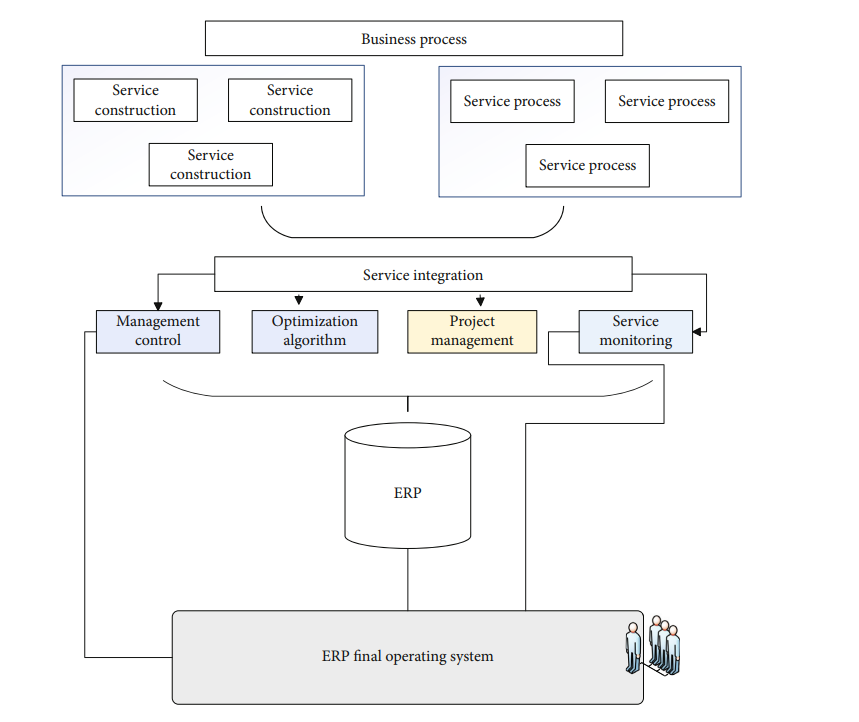
\includegraphics[width=1\linewidth]{img/ERP system framework hierachy.png}
    \caption{ERP System Framework Hierarchy}
    \label{fig:enter-label}
\end{figure}
\par{The diagram shows how an ERP system interprets the defined business process and how it processes this information to generate an effective output. The services that occur during the business process are integrated with a system that monitors, optimizes, and manages these processes and in turn a completed ERP system is created. }
\subsection{Features of ERP Systems}
\par{There are various features that make up an ERP system, however there is no set standard for what an ERP system must be able to functionally do as ERP systems are configured for the need of the company it is built for. However, generally ERP systems can potentially have any of the following features that are discussed and examined below:}
\subsubsection{Financial Management}
\subsubsection{Human Resources Management}
\par{Enterprise managers' main concerns in modern times are increasingly intense business competition amongst enterprises and how to draw in the best talent to become part of the workforce, streamline human resources, cut personnel costs, and increase the competitiveness of enterprises; in other words, these enterprise managers believe that the integration of ERP into the HR system has expanded the system's capabilities to encompass enterprise management. The variety of HR services has expanded as well, from payroll accounting and personnel administration to a comprehensive suite of tools that support business decision-making. Planning for human resources, staff appraisal, scheduling, time management, hiring, payroll, training initiatives, and travel administration are some of these topics. They combine to create an effective and highly integrated ERP, together with the financial and production systems \citep{zhao2021research}.

\cite{zhao2021research} proposes a figure showing the impact of ERP systems in increasing the efficiency of HR procedures within a business. The figure can be seen below and proves the worth and effectiveness of implementing this type of system into the HR workforce.}
\begin{figure}[ht!]
    \centering
    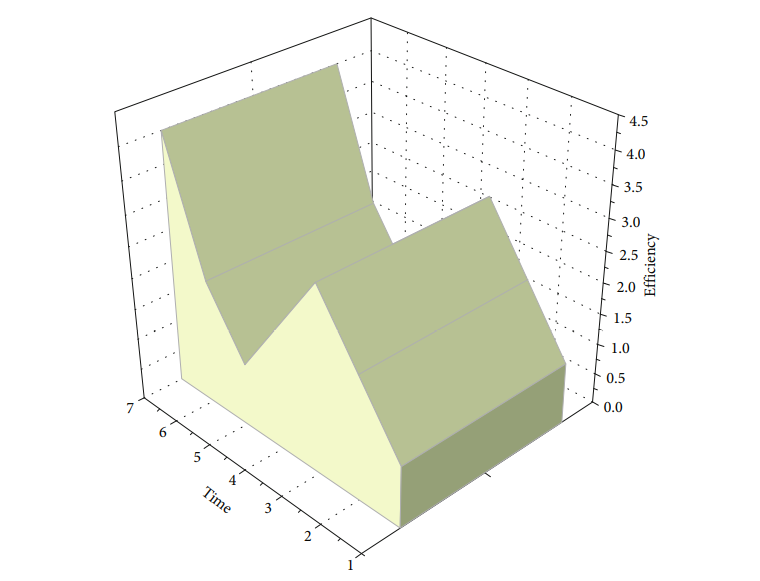
\includegraphics[width=1\linewidth]{img/Human resource management system optimization rate..png}
    \caption{Human resource management system optimization rate}
    \label{fig:enter-label}
\end{figure}
\subsubsection{Supply Chain Management}
\par{The ERP's supply chain component manages all retail operations, including shipments, receipts, issues, and quality control. If you work for a manufacturer, wholesaler, or retailer, managing your inventory is essential to keeping expenses under control and guaranteeing the seamless running of your company. The core functions of every organisation, stock management and valuation, require a significant investment of time and money. Every item's lot-by-lot stock is kept track of, and several computerised information reports are offered to monitor stock movement \citep{ahlawat2017role}.

The ERP supply chain activities include determining the amount of inventory needed, establishing goals, receiving and delivering goods, maintaining materials in stock subsections, categorising every product, supplying materials to the fabrication department, and fully documenting supplier rejections. Additionally, it offers alternatives and strategies for restocking, keeps track of item usage, reconciles inventory balances, and reports the state of inventory \citep{ahlawat2017role}.}
\subsubsection{Customer Relationship Management (CRM)}
\par{The phrase "customer relationship management (CRM)" refers to the capacity to continuously engage with customers across a range of channels; it offers the frameworks necessary for businesses to grow and improve their customer offerings and draw in new ones. Companies are now more interested in knowing their customers and interacting with them in order to seize opportunities and overcome obstacles as a result of the growing rivalry in the business world \citep{kostojohn2011crm}.

Early in the 1990s, CRM was created with the purpose of managing sales teams and direct marketing, as well as preserving consumer data and reaching their preferences from past purchases and conversations \citep{bygstad2013social}. CRM was created to provide a range of essential tools that could be used by businesses of all sizes and in a variety of industries. These tools would enable them to monitor, manage, and share customer data \citep{smilansky2015select}, aid salespeople and marketers in examining the behaviour of their clients, and add value to the company through the use of both human and technological resources \citep{bibiano2014initial}. Therefore, businesses become more competitive, maximise revenues, decrease effort duplication, improve the effectiveness of information storage, make it available to all employees, and provide a single overview to partners and customers. CRM systems comprise the techniques, tools, and capacities that assist an organisation in managing its customer relationship. A significant portion of this work is closely related to the advancement of information and communication technology, which allows businesses to gather the most data possible about their clients' behaviour, contact details, and other characteristics. It also gives them access to efficient tools and methods for managing this data. Thus, the concept of CRM refers to the ability for businesses to better manage their clientele by implementing dependable systems, processes, and procedures that enable them to obtain the most data about their clientele and interact with them for business objectives in order to obtain specific information that aids in the targeting of goods, services, and new markets \citep{ronchi2009eculture}.}
\subsubsection{Project Management}
\subsubsection{Inventory Management}
\par{Real-time data on inventory levels and values, encompassing stock on order, raw materials, ongoing work, and completed products, is provided by ERP software. The ERP inventory component handles all aspect of a company's stock-related operations. An inventory management module is a tool that makes collecting information in the inventory department or warehouse quicker and can assist you in keeping the right amount of stock on hand \citep{ahlawat2017role}.

The supply and demand sides benefit from the application of an inventory management methodology. Inventory management can improve the speed of delivery and stabilise interactions with clients for the supply side. On the demand side, it also lessens the impact of inventory on financial resources, lowers the possibility of material deficits, and quickens the supply chain's reaction time \citep{zhao2021research}.

\cite{zhao2021research} proposes two a flow charts that symbolise the functioning of production, inventory, procurement, and the payment process within an ERP system. This example can be further generalised and seen as a general flow chart of how and ERP system technically and practically functions within a given component of the system which in this case is inventory management. Both these flow charts can be studied below:}
\begin{figure}[ht!]
    \centering
    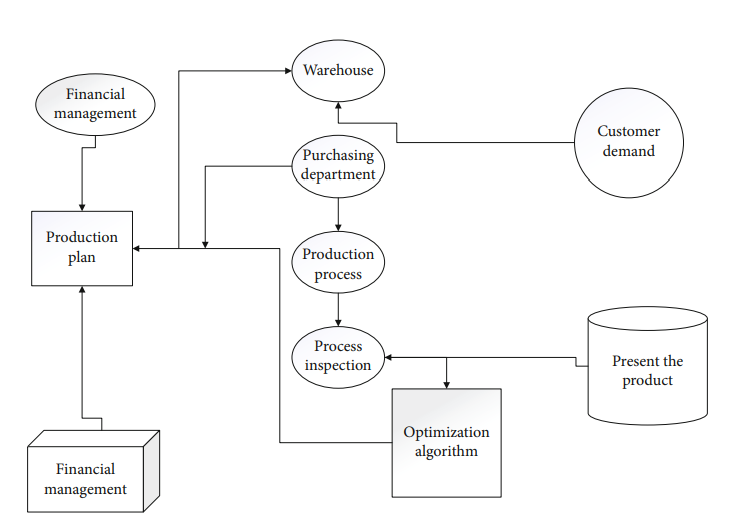
\includegraphics[width=1\linewidth]{img/rename flow chart of company's inventory and production.png}
    \caption{Flow chart of the company’s production and inventory business based on ERP system}
    \label{fig:enter-label}
\end{figure}
\begin{figure}[ht!]
    \centering
    \includegraphics[width=1\linewidth]{img/Flow chart of the company’s ERP-based procurement and payment process.png}
    \caption{Flow chart of the company’s ERP-based procurement and payment process}
    \label{fig:enter-label}
\end{figure}
\par{Within this basic examples we can see how the business process would hypothetically flow and how data moves to and from a database storing the information necessary to produce some sort of return. This concept can be applied throughout various modules of an ERP system. Each function is always user input that is processed, stored in a database, and then an output that is once again returned to the user.}
\subsubsection{Sales and Marketing}
\subsubsection{Business Intelligence (BI)}
\subsubsection{E-commerce}
\subsection{Competition within the ERP System Industry}
\subsection{Components of an Industry Approved Software System}
\subsection{Components of an Industry Approved ERP System}

\section{Implementation of ERP Systems}
\par{The seven main steps in the ERP deployment process include business process analysis, software installation, data migration, software performance testing, user training, complete deployment, and post-implementation support \citep{ly2020definitive}. These main key steps are examined in greater depth in the sections that follow.}
\subsubsection{Business Process Research and Requirements Gathering}
\par{The first step in the ERP implementation procedure is to define the needs, goals, and scope of the ERP within the specified business' process. Building a team that can work on the ERP implementation project from beginning to end is also necessary \citep{wetherbe2006information}. Within the team there would mainly be two roles, software developers and the sub roles that preside within this overarching role, as well as business analysts that are responsible for documenting and understanding the business process and how it will be converted into an ERP system. This step within the implementation process is largely the responsibility of the business analysts. The responsibilities of the business analyst within this step of the process would be as follows \citep{yusuf2004enterprise}:}
\begin{itemize}
    \item Analyse, record, and describe an organisation's current procedures. 
    \item Look for significant difficulties, process waste, and customer-focused problems.
    \item Establish clear objectives for an ERP deployment that are connected to the major success areas, and quantify them precisely.
    \item Create a cost budget and a solid timetable.
\end{itemize}
\subsubsection{Software Installation}
\par{Following the first step's creation of new procedure flows, the team should have a new business process plan in place. The architecture and infrastructure for software, such as the data store, data presentation, and internet accessibility, will be installed and constructed by the software developers who have recieved the business requirements from the business analyst.}
\subsubsection{Data Migration}
\par{In this stage, all data is transferred to a new software platform. Before the data is transferred to a new site, it should all be reviewed and adjusted to ensure a smooth mapping process. Data mapping between the previous and new store locations, data transfer, and the configuration of a new data storage location are all included in this stage.}
\subsubsection{Testing}
\par{All data interfaces, functionality, and real-time data transactions are tested by the quality engineer. Users need to make sure that information is accurately moving between various departments and that the system is functionally sound. The testing process is important to ensure that no edge cases arise during the use of the deployed system and that the system behaves as predicted.}
\subsubsection{User Training}
\par{Personnel react to change management, and user training relies on the intricate nature of the ERP program. Up to 56 percent of ERP deployment cases after go live result in production halts under training.}
\subsubsection{Final Deployment}
\par{Depending on the scale of the ERP software and the assets available, the organisation might select one of the following three ways:}
\begin{itemize}
    \item Big-Bang Method: A one-day switch from the outdated to the updated software. This method is quick and inexpensive, but any inefficiency in deployment could lead to a serious issue during use.
    \item Phased Approach: A longer-term, function- or unit-specific phased transition.
    \item Parallel Operation Approach: In order to reduce risk, users use both new and old systems simultaneously.
    This method has greater operational expenses for the two platforms and necessitates more time for repetition of work.
\end{itemize}
\subsubsection{Support}
\par{Performance review of ERP projects is crucial and should be done for the duration of the project. Key performance indicators that can be compared are as follows:}
\begin{itemize}
    \item Real implementation costs compared to the budgeted amount
    \item The return on investment for the project
    \item The assessment of mistakes or human errors
    \item The efficiency of the supply chain and production
    \item The satisfaction of customers and their willingness to continue working with the development company
\end{itemize}
\subsection{ERP Implementation Time}
\par{Once the software system is launched, an ERP system implementation project may take anywhere from three months to several years to complete and fully implement to a point where both client and development company are satisfied \citep{sankar2006implementation}. The size of the organisation, the volume of data, the number of users, and the resources all affect how long the ultimate project implementation takes \citep{pelphrey2015directing}.}
\subsection{Critical Competencies for Software Development}

\section{The Information Technology Industry}
\subsection{Challenges within the Information Technology Industry}
\subsection{Challenges Exclusive to Developing Nations}
\subsubsection{The Purpose of a University}
\subsection{Developing Nations vs. The Rest of the World}

\section{The Value Chain}
\subsection{People}
\subsection{Processes}
\subsection{Technology}
\subsubsection{Hardware}
\subsubsection{Software}
\subsubsection{Infrastructure}
\subsection{The Economic Viability of Academic and Industry Partnership}
\subsection{Industry Offering Resources to Universities}

\section{Commercialization of Software}
\subsection{Methods of Commercialization}
\subsubsection{Recommendation}

\section{Students in Industry}
\subsection{Advantages}
\subsection{Threats}
\subsection{Similar Projects}

\section{Project Management Methodologies}
\subsection{Software Development Management Methodologies}
\subsection{Recommendations}

\section{Artefact}
\subsection{Methods for Measuring Artefact Success}
\subsection{Methods for Measuring Artefact Functionality}
\subsection{TAM Model}